% Thesis report: Bangla toxic comment detection.
% Compiles with pdfLaTeX (fastest, Overleaf default) or XeLaTeX. References use BibTeX.
% Charts are drawn by make_figures.py into figures/.

\documentclass[12pt]{report}

% ---------------------------------------------------------------------------
% Details for the title page and certificate. Check each one.
% ---------------------------------------------------------------------------
\newcommand{\thesistitle}{Detecting Toxic Comments in Bangla Social Media: A Comparative Study of Fine-tuned Transformers, Zero-shot Large Language Models and Lexicon-based Filtering}
\newcommand{\studentA}{MONTASIR MAMUN SAGOR}
\newcommand{\studentAid}{12008025}
\newcommand{\degree}{MASTER OF SCIENCE}
\newcommand{\coursename}{In Partial Fulfillment of the Requirements for the Degree of}
\newcommand{\department}{DEPARTMENT OF COMPUTER SCIENCE AND ENGINEERING}
\newcommand{\university}{COMILLA UNIVERSITY, CUMILLA-3506}
\newcommand{\supervisor}{Khairun Nahar}
\newcommand{\supervisorrank}{Assistant Professor}
\newcommand{\chairman}{Khairun Nahar}
\newcommand{\chairmanrank}{Assistant Professor}
\newcommand{\submissiondate}{November 2026}

% ---------------------------------------------------------------------------
% Fonts. pdfLaTeX (the Overleaf default) is the fastest to compile. TeX Gyre Termes is a
% Times New Roman clone.
% ---------------------------------------------------------------------------
\usepackage{iftex}
\ifPDFTeX
  \usepackage[T1]{fontenc}
  \usepackage[utf8]{inputenc}
  \usepackage{tgtermes}
\else
  \usepackage{fontspec}
  \setmainfont{TeX Gyre Termes}
\fi

\usepackage{graphicx}
\graphicspath{{figures/}}
\usepackage{float}
\usepackage{amsmath,amssymb,amsfonts}
\usepackage{textcomp}
\usepackage[table]{xcolor}
\usepackage{array,multirow,booktabs,tabularx}
\usepackage{url}
\usepackage{ragged2e}
\usepackage{enumitem}
\usepackage{caption}
\usepackage{tikz}
\usetikzlibrary{arrows.meta,positioning,shapes.geometric,fit}
\usepackage[hidelinks]{hyperref}

% natbib + BibTeX compiles much faster than biblatex + Biber on the free Overleaf plan
\usepackage[numbers,sort&compress]{natbib}
\renewcommand{\bibname}{References}

\usepackage[parfill]{parskip}
\usepackage{geometry}
\usepackage{sectsty}
\chapterfont{\centering}
\geometry{
  paper=a4paper,
  top=1in,
  bottom=1in,
  left=1.2in,
  right=0.8in,
  headheight=0.75cm,
  footskip=1.5cm,
  headsep=0.75cm,
}
\linespread{1.5}

\begin{document}

% ===========================================================================
% Title page
% ===========================================================================
\begin{titlepage}
  \centering
  
\includegraphics[height=4cm,width=4cm]{unilogo.png}\par
  \vspace{0.3cm}
  {\huge\bfseries Comilla University\par}
  \vspace{0.5cm}
  {\scshape\Large\bfseries \thesistitle\par}
  \vspace{0.45cm}
  {\scshape\Large\bfseries A THESIS REPORT\par}
  {\scshape\Large\bfseries \textit{Submitted By}\par}
  {\Large\textbf{\studentA}}\par
  {\Large{ID: \studentAid}}\par
  \vspace{0.35cm}
  {\large\textbf{\textit{\coursename}}}\par
  {\Large\textbf{\degree}}\par
  \vspace{0.1cm}
  {\large\textbf{IN}}\par
  {\large\textbf{\department}\par}
  \vspace{0.45cm}
  {\Large\textbf{\university}}\par
  \vspace{0.35cm}
  {\Large\bfseries \submissiondate}\par
\end{titlepage}

% ===========================================================================
% Certificate
% ===========================================================================
\newpage
\pagenumbering{gobble}
\begin{center}
  \large\textbf{BONAFIDE CERTIFICATE}
\end{center}

This is to certify that the thesis entitled \textbf{``\thesistitle''} is submitted by \studentA{}, who carried out the work under my supervision. This is the bonafide work.

\vspace{2cm}

\noindent
\begin{tabular}{l@{\hspace{3cm}}l}
Signature & Signature \\[1.5cm]
\makebox[5cm]{\dotfill} & \makebox[5cm]{\dotfill} \\
\chairman & \supervisor \\
\textbf{Chairman of the Exam Committee} & \textbf{Supervisor} \\
\chairmanrank & \supervisorrank \\
Department of CSE & Department of CSE \\
Comilla University, Cumilla. & Comilla University, Cumilla. \\
\end{tabular}

\newpage
\pagenumbering{Roman}

% ===========================================================================
% Abstract
% ===========================================================================
\chapter*{Abstract}
\addcontentsline{toc}{chapter}{Abstract}
\justifying

Toxic and abusive comments are widespread on Bangla social media, yet most moderation tools are built for English. This thesis compares four ways of detecting toxic Bangla comments automatically: a word-list (lexicon) filter, two fine-tuned transformer models (the Bangla-specific BanglaBERT and the multilingual XLM-RoBERTa), and a large language model (LLM) used zero-shot, without any task-specific training.

The study uses the Multi-labeled Bengali Toxic Comments dataset. Its six toxicity labels (vulgar, hate, religious, threat, troll and insult) are merged into one binary label, giving 15,913 comments after cleaning, of which 53.2\% are toxic. All methods are scored on the same stratified test set of 3,183 comments. Model selection uses a separate validation split, so the test set is used only for final scores. Each fine-tuned model is trained three times with different random seeds, and a learning curve measures how much labelled data the models need.

XLM-RoBERTa achieves the best result, with a weighted F1-score of 0.943 $\pm$ 0.001, ahead of BanglaBERT at 0.928 $\pm$ 0.003, and it stays ahead at every amount of training data. The zero-shot LLM (Qwen, accessed through the Groq API) reaches an F1-score of 0.768. It is highly precise when it flags a comment as toxic (precision 0.97) but misses 41\% of toxic comments, and it runs about 70 times slower than the fine-tuned models. The English word-list filter fails almost completely (F1 0.299) because it does not recognise Bangla words.

The results show that fine-tuning a pretrained transformer on a modest amount of labelled Bangla data clearly outperforms both lexicon filtering and zero-shot prompting of a general-purpose LLM, while also being far cheaper to run. A multilingual model pretrained on a very large corpus can outperform a smaller language-specific model. The thesis also provides a reproducible pipeline that runs on free cloud GPUs, and a web demo.

\textbf{Keywords:} Bangla, toxic comment detection, hate speech, BanglaBERT, XLM-RoBERTa, large language models, zero-shot classification, low-resource NLP.

% ===========================================================================
% Acknowledgement
% ===========================================================================
\chapter*{Acknowledgement}
\addcontentsline{toc}{chapter}{Acknowledgement}

First and foremost, I thank the Almighty Allah for His blessings, which gave me the health and determination to complete this thesis.

I express my sincere gratitude to my supervisor, \textbf{\supervisor}, for her guidance, careful review and constant encouragement throughout this work on \textbf{``\thesistitle''}.

I thank the authors of the Multi-labeled Bengali Toxic Comments dataset for making their data publicly available, and the developers of the open-source tools this work builds on, including Hugging Face Transformers, PyTorch and scikit-learn. I also acknowledge Google Colab for free GPU access and Groq for free API access to the language model used in this study.

% If your university requires it, state the use of AI tools here, for example:
% "AI-based tools were used to assist with parts of the software implementation; all
%  experimental design, analysis and conclusions are my own."

Finally, I thank my family and friends for their support and patience throughout this journey.

% ===========================================================================
% Front matter lists
% ===========================================================================
\newpage
\renewcommand*\contentsname{Table of Contents}
\tableofcontents
\listoffigures
\listoftables

\chapter*{List of Abbreviations}
\addcontentsline{toc}{chapter}{List of Abbreviations}
\begin{tabular}{@{}ll@{}}
API     & Application Programming Interface \\
BERT    & Bidirectional Encoder Representations from Transformers \\
F1      & Harmonic mean of precision and recall \\
FN / FP & False Negative / False Positive \\
GPU     & Graphics Processing Unit \\
LLM     & Large Language Model \\
MLM     & Masked Language Modelling \\
NLP     & Natural Language Processing \\
TN / TP & True Negative / True Positive \\
XLM-R   & XLM-RoBERTa (Cross-lingual Language Model, RoBERTa architecture) \\
\end{tabular}

\clearpage
\pagenumbering{arabic}

% ===========================================================================
% Chapters. If a full compile times out on the free Overleaf plan, comment out
% some \input lines, compile, then uncomment them and compile again.
% ===========================================================================
\chapter{Introduction}
\justifying

\section{Background}

Bangla (Bengali) is spoken by more than 250 million people and is one of the most widely spoken languages in the world. A rapidly growing share of Bangla speakers use social media platforms such as Facebook and YouTube, where they post and comment in their own language. Alongside constructive discussion, these platforms host a large volume of toxic content: insults, vulgar language, threats, trolling, and hate directed at people because of their religion or identity.

Toxic comments harm the people they target, discourage participation in online discussion and can contribute to offline conflict. Platforms therefore rely on automatic moderation to flag harmful content, because the volume of comments is far too large for human moderators alone. Such systems have been developed mainly for English and a few other high-resource languages \cite{schmidt2017survey,fortuna2018survey}. For Bangla, labelled datasets and well-tested tools are much scarcer, which makes it a \emph{low-resource} language for this task.

Recent progress in natural language processing (NLP) offers two broad routes to closing this gap. The first is \emph{fine-tuning} a pretrained transformer model \cite{vaswani2017attention,devlin2019bert} on a labelled dataset, either a Bangla-specific model such as BanglaBERT \cite{sarker2020banglabert} or a multilingual model such as XLM-RoBERTa \cite{conneau2020xlmr}. The second is to use a \emph{large language model} (LLM) through prompting alone, without any task-specific training \cite{brown2020gpt3}. Simpler approaches, such as filtering comments against a list of offensive words, are still widely used in practice because they are easy to deploy.

\section{Problem Statement}

It is not yet clear which of these approaches works best for detecting toxic Bangla comments, or what trade-offs each one involves. Fine-tuning requires labelled data and GPU training, whereas zero-shot LLMs need no training data but are slower and depend on an external service. Language-specific models are trained on Bangla text alone, whereas multilingual models are trained on far more data spread across many languages. A word-list filter needs neither data nor training, but it may not cope with Bangla's rich vocabulary and spelling variation. A fair, like-for-like comparison of these approaches on the same Bangla data is needed to guide practitioners.

\section{Motivation}

This work is motivated by three observations. First, Bangla users deserve the same protection from online abuse as speakers of high-resource languages. Second, the rise of general-purpose LLMs raises a practical question: is it still worth collecting labelled data and fine-tuning models, or can a prompted LLM do the job? Third, many studies report results from a single training run, which makes it hard to tell whether a difference between two models is real or caused by random variation. A careful evaluation with repeated runs and a strict separation between validation and test data gives more trustworthy conclusions.

\section{Research Questions}

This thesis addresses the following research questions:

\begin{enumerate}[label=\textbf{RQ\arabic*.}, leftmargin=*]
  \item How accurately can fine-tuned transformer models detect toxic Bangla comments?
  \item Does a Bangla-specific pretrained model (BanglaBERT) outperform a multilingual one (XLM-RoBERTa)?
  \item How does a zero-shot large language model compare with fine-tuned models in accuracy and speed?
  \item Is a word-list (lexicon) filter an adequate baseline for Bangla?
  \item How does the performance of fine-tuned models change with the amount of training data?
\end{enumerate}

\section{Contributions}

The main contributions of this thesis are:

\begin{itemize}
  \item A controlled comparison of four detection approaches, namely a lexicon filter, BanglaBERT, XLM-RoBERTa and a zero-shot LLM, all scored on the same held-out test set of 3,183 Bangla comments.
  \item A leakage-free evaluation protocol, with a separate validation split for model selection, three training runs per model with different random seeds, and a learning-curve analysis.
  \item An analysis of the trade-offs between accuracy, error types and inference speed, with practical recommendations for Bangla content moderation.
  \item An open, reproducible implementation that runs on free cloud GPUs (Google Colab), together with an interactive web demo.
\end{itemize}

\section{Thesis Organization}

The rest of this thesis is organised as follows.

\textbf{Chapter 2: Literature Review} surveys work on toxic and hate speech detection, Bangla datasets and models, pretrained transformers, and LLM-based classification.

\textbf{Chapter 3: Methodology} describes the dataset, preprocessing, the four approaches, the training setup and the evaluation protocol.

\textbf{Chapter 4: Results and Discussion} presents and analyses the experimental results.

\textbf{Chapter 5: Conclusion and Future Work} summarises the findings, limitations and directions for future research.

\chapter{Literature Review}
\justifying

This chapter reviews four areas that this thesis builds on: automatic detection of toxic and hateful text in general, work specific to Bangla, pretrained transformer language models, and the use of large language models for classification.

\section{Toxic and Hate Speech Detection}

Automatic detection of abusive language has been studied extensively for English. Surveys by Schmidt and Wiegand \cite{schmidt2017survey} and Fortuna and Nunes \cite{fortuna2018survey} describe how early systems relied on hand-crafted features such as word lists, n-grams and sentiment scores, fed into classical classifiers. Davidson et al. \cite{davidson2017automated} showed that separating hate speech from merely offensive language is difficult, and that systems relying on the presence of particular words produce many errors: offensive words appear in harmless contexts, and hateful messages can avoid explicit slurs. These findings motivate approaches that model the meaning of a whole sentence rather than individual words.

\section{Toxic and Hate Speech Detection in Bangla}

Bangla has received growing attention in recent years. Ishmam and Sharmin \cite{ishmam2019hateful} collected comments from public Facebook pages and classified hateful speech using machine learning and recurrent neural networks. Romim et al. \cite{romim2021hate} released a dataset of around 30,000 Bangla comments annotated for hate speech, with baseline results from classical and deep learning models. The same group later published BD-SHS \cite{romim2022bdshs}, a larger benchmark that also records the social context and target of hate speech. Karim et al. \cite{karim2021deephateexplainer} applied transformer models, including multilingual BERT and XLM-RoBERTa, to Bangla hate speech and added explanations of the model decisions.

Belal et al. \cite{belal2023toxic} introduced the Multi-labeled Bengali Toxic Comments dataset used in this thesis. Each comment is annotated with six toxicity types: vulgar, hate, religious, threat, troll and insult. They proposed a two-stage approach that first decides whether a comment is toxic and then identifies the toxicity types, and reported a binary accuracy of 89.42\% for the first stage.

\section{Pretrained Transformer Language Models}

The transformer architecture \cite{vaswani2017attention} and BERT \cite{devlin2019bert} established the now-standard approach of pretraining a language model on large unlabelled corpora and then fine-tuning it on a specific task. RoBERTa \cite{liu2019roberta} improved the pretraining recipe. XLM-RoBERTa \cite{conneau2020xlmr} applied this recipe to 2.5 TB of filtered web text in 100 languages, including Bangla, and showed strong cross-lingual performance, notably for low-resource languages.

Two Bangla-specific models share the name BanglaBERT. Sarker \cite{sarker2020banglabert} released a BERT-base model (\texttt{sagorsarker/bangla-bert-base}) pretrained on Bangla Wikipedia and the Bangla portion of OSCAR, which is the model used in this thesis. Bhattacharjee et al. \cite{bhattacharjee2022banglabert} later released a separate model (\texttt{csebuetnlp/banglabert}) pretrained with the ELECTRA objective on a larger Bangla corpus, together with a benchmark of Bangla language understanding tasks.

\section{Large Language Models for Classification}

Large language models can carry out many tasks from a natural-language instruction alone, without task-specific training, a setting known as zero-shot learning \cite{brown2020gpt3}. This is attractive for low-resource languages, where labelled data is scarce. However, LLMs are trained mostly on English text, are expensive to run, and their behaviour on sensitive tasks such as content moderation depends heavily on their safety tuning. Open-weight models such as the Qwen3 family \cite{yang2025qwen3} are multilingual and can be accessed through low-latency inference services.

\section{Research Gap}

Previous Bangla studies usually evaluate one family of methods, report a single training run, and rarely compare fine-tuned models with zero-shot LLMs on the same test data. This thesis addresses that gap by comparing a lexicon filter, a Bangla-specific transformer, a multilingual transformer and a zero-shot LLM under one controlled protocol, with repeated runs, leakage-free model selection and an analysis of speed as well as accuracy.

\chapter{Methodology}
\justifying

This chapter describes the research design, the dataset and its preparation, the four detection approaches, the training configuration and the evaluation protocol.

\section{Research Design}

The study is an empirical, comparative experiment. All four approaches classify each comment as \emph{toxic} or \emph{non-toxic}, and all are scored on exactly the same held-out test set. Figure~\ref{fig:pipeline} summarises the pipeline.

\begin{figure}[!htb]
  \centering
  \resizebox{\textwidth}{!}{%
  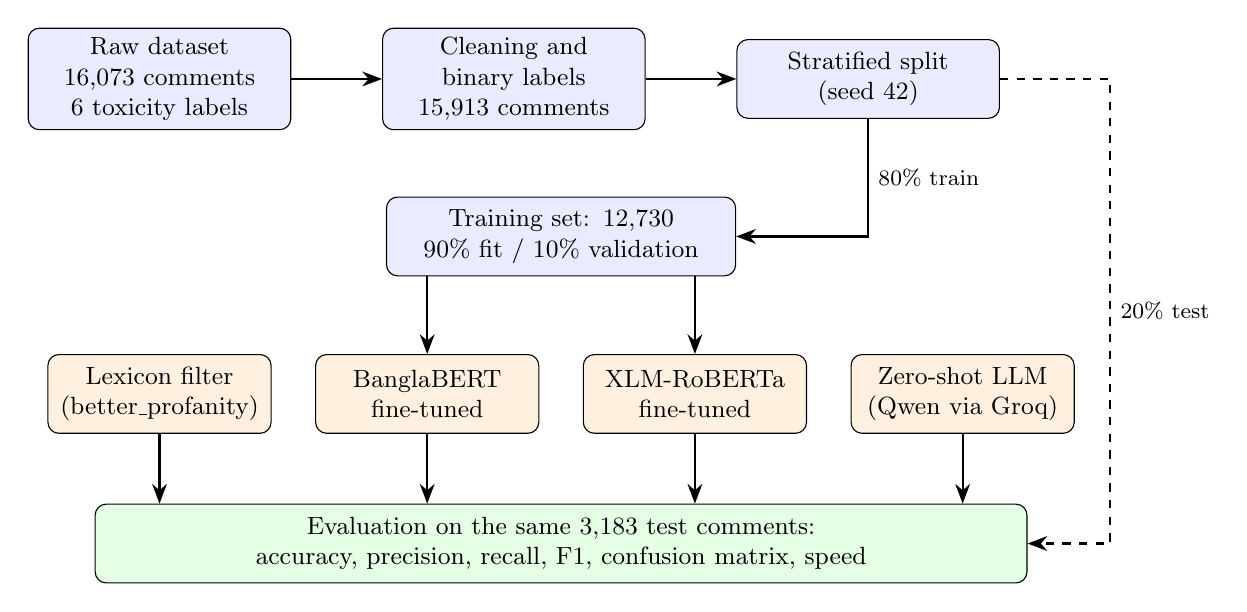
\begin{tikzpicture}[
      box/.style={draw, rounded corners, align=center, minimum height=1cm, text width=3.1cm, font=\small},
      databox/.style={box, fill=blue!8},
      modelbox/.style={box, fill=orange!12, text width=2.6cm},
      resultbox/.style={box, fill=green!10, text width=11.6cm},
      arrow/.style={-{Stealth[length=2.5mm]}, thick}]
    \node[databox] (raw)   at (0,0)   {Raw dataset\\16,073 comments\\6 toxicity labels};
    \node[databox] (clean) at (4.5,0) {Cleaning and\\binary labels\\15,913 comments};
    \node[databox] (split) at (9,0)   {Stratified split\\(seed 42)};
    \node[databox, text width=4.2cm] (train) at (5.1,-2.0) {Training set: 12,730\\90\% fit / 10\% validation};

    \node[modelbox] (lex) at (0,-4.0)    {Lexicon filter\\(better\_profanity)};
    \node[modelbox] (bb)  at (3.4,-4.0)  {BanglaBERT\\fine-tuned};
    \node[modelbox] (xr)  at (6.8,-4.0)  {XLM-RoBERTa\\fine-tuned};
    \node[modelbox] (llm) at (10.2,-4.0) {Zero-shot LLM\\(Qwen via Groq)};

    \node[resultbox] (eval) at (5.1,-5.9) {Evaluation on the same 3,183 test comments:\\accuracy, precision, recall, F1, confusion matrix, speed};

    \draw[arrow] (raw) -- (clean);
    \draw[arrow] (clean) -- (split);
    \draw[arrow] (split.south) |- node[pos=0.25, right, font=\footnotesize] {80\% train} (train.east);
    \draw[arrow] (bb.north |- train.south) -- (bb.north);
    \draw[arrow] (xr.north |- train.south) -- (xr.north);
    \draw[arrow, dashed] (split.east) -- ++(1.4,0) |- node[pos=0.25, right, font=\footnotesize] {20\% test} (eval.east);
    \foreach \m in {lex,bb,xr,llm} \draw[arrow] (\m.south) -- (\m.south |- eval.north);
  \end{tikzpicture}}
  \caption{Experimental pipeline. Only the two fine-tuned models use the training set. The lexicon filter and the LLM need no training. All four approaches are scored on the same held-out test set (dashed arrow).}
  \label{fig:pipeline}
\end{figure}

\section{Dataset}

The experiments use the \textbf{Multi-labeled Bengali Toxic Comments} dataset of Belal et al. \cite{belal2023toxic}, collected from Bangla social media. It contains 16,073 comments. Each comment carries six binary labels; Table~\ref{tab:rawlabels} shows how often each label occurs. A comment can carry several labels at once, and comments with no label are non-toxic.

\begin{table}[H]
  \centering
  \caption{Occurrences of each toxicity label in the raw dataset (16,073 comments). A comment can carry more than one label.}
  \label{tab:rawlabels}
  \begin{tabular}{lrl}
    \toprule
    \textbf{Label} & \textbf{Comments} & \textbf{Description} \\
    \midrule
    Insult    & 2,719 & Insulting or demeaning a person \\
    Vulgar    & 2,505 & Obscene or sexually explicit language \\
    Hate      & 1,898 & Hatred towards a person or group \\
    Troll     & 1,643 & Mocking or provocative trolling \\
    Threat    & 1,419 & Threats of violence or harm \\
    Religious & 1,418 & Attacks on religion or religious groups \\
    \bottomrule
  \end{tabular}
\end{table}

\section{Preprocessing and Label Construction}

The data was prepared with a small conversion script in the following steps:

\begin{enumerate}
  \item \textbf{Binary labelling.} A comment is labelled \emph{toxic} (1) if \emph{any} of the six labels is set, and \emph{non-toxic} (0) otherwise. This turns the task into binary classification, which matches the typical moderation decision of whether to flag a comment.
  \item \textbf{Cleaning.} Leading and trailing whitespace was removed, and empty comments were dropped.
  \item \textbf{De-duplication.} Exact duplicate comments were removed, keeping the first occurrence. This prevents the same text from appearing in both the training and test sets, which would inflate the scores.
\end{enumerate}

No further normalisation, such as stemming or stop-word removal, was applied. The transformer models use their own subword tokenisers, which work best on raw text.

After preprocessing, 15,913 comments remain: 8,459 toxic (53.2\%) and 7,454 non-toxic (46.8\%), so the two classes are reasonably balanced (Figure~\ref{fig:classdist}). Comments are short. They contain 14.3 words (80 characters) on average, the median is 11 words, and the longest comment has 238 words. Figure~\ref{fig:lengths} shows that toxic and non-toxic comments have very similar length distributions, so comment length alone gives little clue to the label.

\begin{figure}[H]
  \centering
  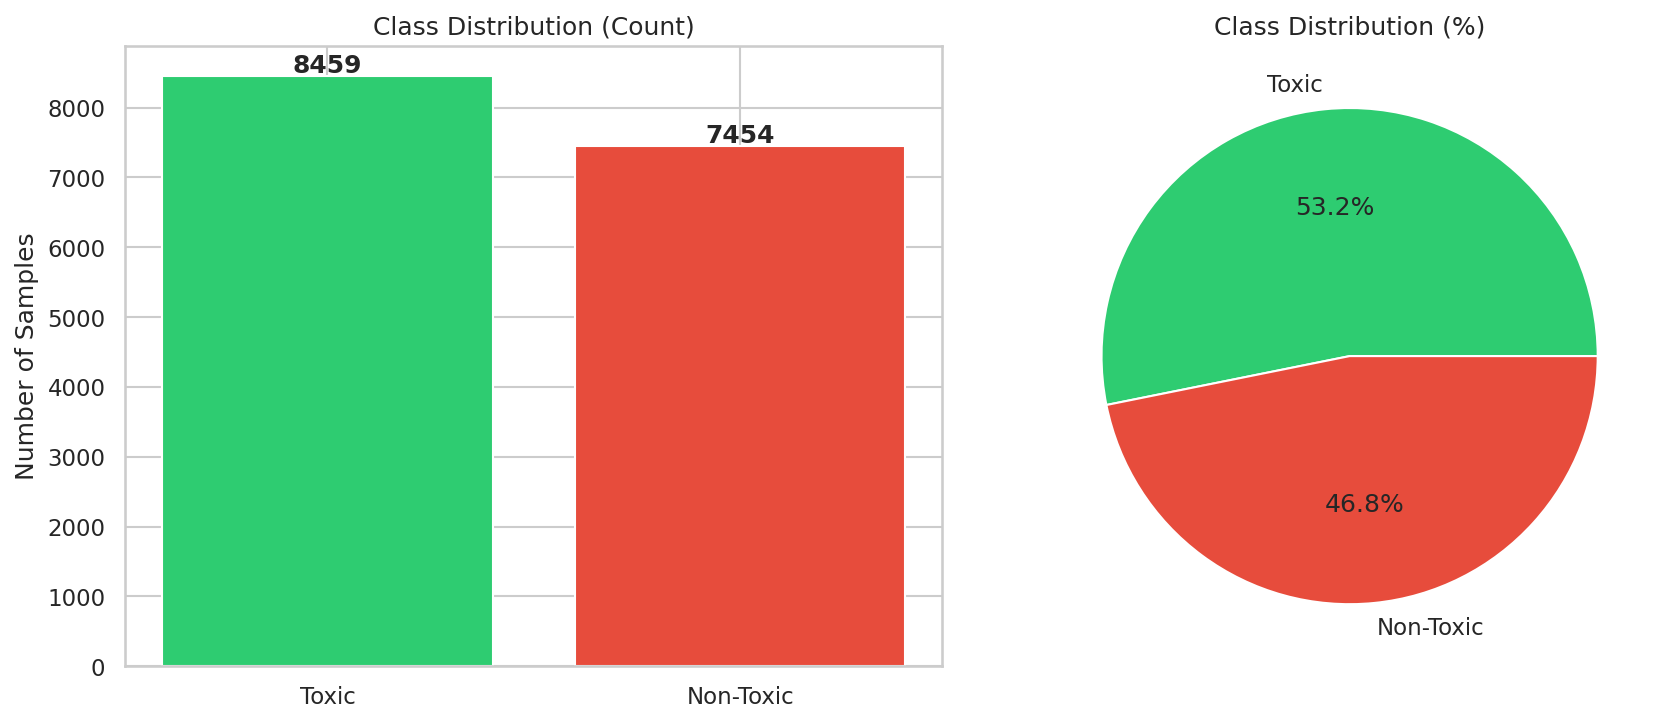
\includegraphics[width=0.9\textwidth]{class_distribution.png}
  \caption{Class distribution after preprocessing (15,913 comments).}
  \label{fig:classdist}
\end{figure}

\begin{figure}[H]
  \centering
  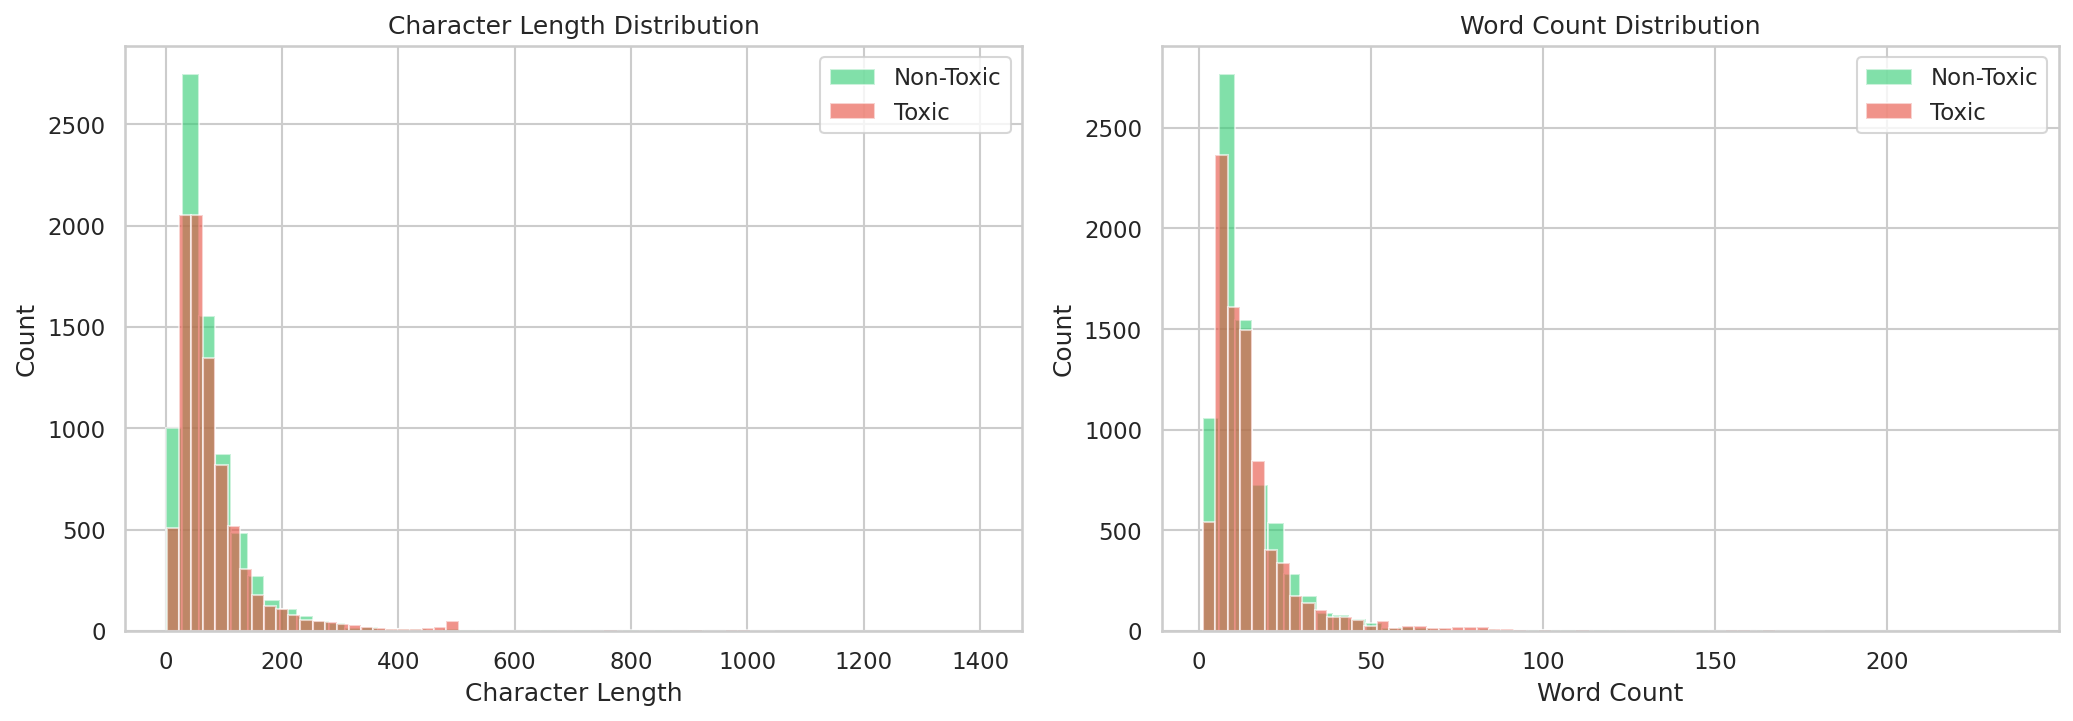
\includegraphics[width=\textwidth]{text_length_distribution.png}
  \caption{Distribution of comment length in characters (left) and words (right) for each class.}
  \label{fig:lengths}
\end{figure}

\section{Data Splitting}

The data was split once with a fixed random seed (42) and stratification by label, so each subset keeps the overall class ratio:

\begin{itemize}
  \item \textbf{Training set:} 12,730 comments (80\%), of which 6,767 are toxic.
  \item \textbf{Test set:} 3,183 comments (20\%), of which 1,692 are toxic and 1,491 non-toxic.
\end{itemize}

For the fine-tuned models, 10\% of the training set (1,273 comments) was further held out as a stratified \textbf{validation set}, leaving 11,457 comments for gradient updates. The validation set is used for early stopping and for choosing the best checkpoint. The test set is used \emph{only} once, to compute the final scores. This avoids a common source of over-optimistic results, where the test set is also used to choose the model. All four approaches are evaluated on the same 3,183 test comments.

\section{Detection Approaches}

\subsection{Lexicon Baseline}

The first baseline is \texttt{better\_profanity} \cite{betterprofanity}, a widely used Python library that flags text containing any word from its built-in profanity list, including common obfuscated spellings. It needs no training. Its list is in English, so it represents the common practice of applying an off-the-shelf filter to a new language without adapting it.

\subsection{BanglaBERT}

BanglaBERT (\texttt{sagorsarker/bangla-bert-base}) \cite{sarker2020banglabert} uses the BERT-base architecture (12 layers, hidden size 768) and was pretrained with masked language modelling on Bangla text only. A linear classification layer is added on top of the \texttt{[CLS]} token representation, and the whole network is fine-tuned on the training data.

\subsection{XLM-RoBERTa}

XLM-RoBERTa (\texttt{xlm-roberta-base}) \cite{conneau2020xlmr} is a multilingual RoBERTa model (12 layers, hidden size 768, about 270 million parameters, most of them in its large 250,000-token vocabulary) pretrained on 2.5 TB of web text in 100 languages. It is fine-tuned in the same way and with the same hyperparameters as BanglaBERT, so the comparison isolates the effect of the pretrained model.

\subsection{Zero-shot Large Language Model}

The LLM baseline uses Qwen (\texttt{qwen/qwen3.8-27b}) \cite{yang2025qwen3}, an open-weight model accessed through the Groq inference API \cite{groqdocs}. The model receives no training examples. Comments are sent in batches of 25, with a fixed instruction asking for one label per comment. Decoding is deterministic (temperature 0), and the model's step-by-step reasoning mode is turned off, so that it returns only the list of labels. A reply is accepted only if it contains exactly one valid label for every comment in the batch; otherwise the batch is retried up to three times.

\section{Training Configuration}

Both transformer models were fine-tuned with the Hugging Face Transformers library \cite{wolf2020transformers} using the settings in Table~\ref{tab:hyper}. They are standard values recommended for fine-tuning BERT-style models \cite{devlin2019bert} and were not tuned further, so that both models are compared under identical conditions.

\begin{table}[H]
  \centering
  \caption{Fine-tuning hyperparameters (identical for both models).}
  \label{tab:hyper}
  \begin{tabular}{ll}
    \toprule
    \textbf{Setting} & \textbf{Value} \\
    \midrule
    Maximum sequence length & 256 tokens \\
    Batch size & 16 \\
    Optimiser & AdamW \\
    Learning rate & $2\times10^{-5}$, linear decay \\
    Warm-up & 10\% of training steps \\
    Weight decay & 0.01 \\
    Maximum epochs & 5 \\
    Early stopping & patience of 2 epochs on validation F1 \\
    Checkpoint selection & best validation F1 (weighted) \\
    Precision & mixed (FP16) \\
    Random seeds & 43, 44, 45 (one per run) \\
    Hardware & NVIDIA T4 GPU (16 GB), Google Colab \\
    \bottomrule
  \end{tabular}
\end{table}

\section{Evaluation Protocol}

\subsection{Metrics}

Predictions are compared with the true labels using accuracy, precision, recall and F1-score. Precision, recall and F1 are averaged over the two classes, with each class weighted by its number of test comments (weighted average). The weighted F1-score is the main metric. Per-class scores, the confusion matrix and the number of false positives (non-toxic comments wrongly flagged) and false negatives (toxic comments missed) are also reported, because the two error types have different costs in moderation.

\subsection{Repeated Runs}

Fine-tuning results vary with the random seed, which controls classifier initialisation and the order of the training data. Each transformer model was therefore trained three times with different seeds, keeping the data splits fixed, and the mean and standard deviation over the three runs are reported. The model from the first run is used for the detailed analysis, such as the confusion matrices, and for the demo.

\subsection{Learning Curve}

To answer RQ5, each transformer model was also trained on the first 25\%, 50\% and 100\% of the (shuffled) training set and evaluated on the full test set.

\subsection{Inference Speed}

Speed is reported as the number of test comments classified per second. For the fine-tuned models, this is measured on the Colab T4 GPU. For the LLM, it includes network round-trips and the pauses required by the free-tier rate limits, so it reflects the practical throughput of this setup rather than the raw speed of the model.

\section{Implementation}

The pipeline is implemented in Python using PyTorch, Hugging Face Transformers \cite{wolf2020transformers} and scikit-learn \cite{pedregosa2011sklearn}. It is organised as six Jupyter notebooks (data exploration, the lexicon baseline, BanglaBERT, XLM-RoBERTa, the LLM baseline, and evaluation), backed by a tested Python package and a command-line entry point. All experiments ran on the free tier of Google Colab. Results are stored on Google Drive, and finished runs are detected and skipped automatically, so an interrupted session can resume without repeating work. A web demo built with Gradio lets a user type a Bangla comment and see the predicted label and confidence.

\chapter{Results and Discussion}
\justifying

This chapter presents the results of the four approaches on the common test set, analyses their errors, training behaviour and speed, and then answers the research questions.

\section{Overall Comparison}

Table~\ref{tab:main} summarises the performance of all four approaches, and Figure~\ref{fig:f1bar} compares their F1-scores.

\begin{table}[H]
  \centering
  \caption{Results on the test set (3,183 comments). Fine-tuned models: mean $\pm$ standard deviation over three runs. Precision, recall and F1 are weighted averages. Speed is comments per second.}
  \label{tab:main}
  \small
  \begin{tabular}{lccccr}
    \toprule
    \textbf{Model} & \textbf{Accuracy} & \textbf{Precision} & \textbf{Recall} & \textbf{F1} & \textbf{Speed} \\
    \midrule
    better\_profanity (lexicon) & 0.4684 & 0.2194 & 0.4684 & 0.2989 & 21.4 \\
    LLM, zero-shot (Qwen)$^{*}$ & 0.7748 & 0.8347 & 0.7748 & 0.7681 & 2.6 \\
    BanglaBERT (fine-tuned) & 0.9276 $\pm$ 0.0035 & 0.9279 & 0.9276 & 0.9276 $\pm$ 0.0035 & 183.3 \\
    \textbf{XLM-RoBERTa (fine-tuned)} & \textbf{0.9430 $\pm$ 0.0013} & \textbf{0.9433} & \textbf{0.9430} & \textbf{0.9430 $\pm$ 0.0013} & 177.2 \\
    \bottomrule
  \end{tabular}

  \vspace{0.2cm}
  \footnotesize $^{*}$Scored on the 3,033 of 3,183 test comments that it classified before the daily API limit was reached (Section~\ref{sec:llm}).
\end{table}

\begin{figure}[H]
  \centering
  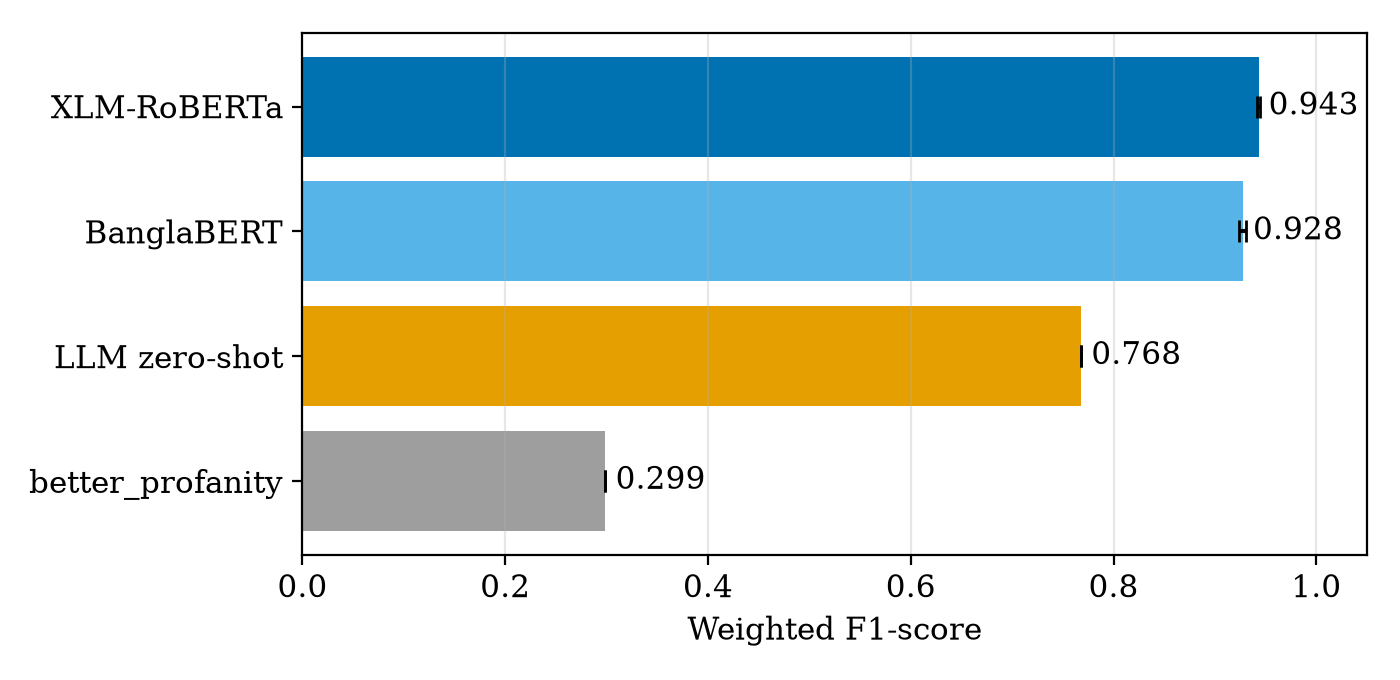
\includegraphics[width=0.85\textwidth]{f1_comparison.png}
  \caption{Weighted F1-score of each approach on the test set. Error bars show the standard deviation over three runs for the fine-tuned models.}
  \label{fig:f1bar}
\end{figure}

The fine-tuned transformers clearly outperform the other two approaches. XLM-RoBERTa is the best model, with an F1-score of 0.943, followed by BanglaBERT at 0.928. The zero-shot LLM is about 16 F1 points behind them, and the lexicon filter barely works. The sections below look at each approach in more detail.

\section{Lexicon Baseline}

The \texttt{better\_profanity} filter reaches an accuracy of 0.468 and an F1-score of 0.299. Its confusion matrix (Figure~\ref{fig:cm}) shows that it labelled every one of the 3,183 test comments as non-toxic, so its accuracy simply equals the share of non-toxic comments in the test set ($1{,}491/3{,}183 = 0.468$). The reason is that its word list contains English words, which almost never occur in Bangla script. This confirms that an off-the-shelf English profanity filter offers no protection for Bangla users, and that toxicity detection needs language-specific resources.

\section{Fine-tuned Transformer Models}

\subsection{Performance and Stability}

The F1-scores of the three BanglaBERT runs were 0.9270, 0.9236 and 0.9321 (mean 0.9276, standard deviation 0.0035). The three XLM-RoBERTa runs scored 0.9412, 0.9444 and 0.9433 (mean 0.9430, standard deviation 0.0013). The gap between the two models (about 1.5 F1 points) is more than four times the larger standard deviation, and every XLM-RoBERTa run scored higher than every BanglaBERT run. The difference is therefore consistent across random seeds, although three runs are too few for a formal significance test. XLM-RoBERTa is also the more stable of the two models. A training run took about 14 minutes for BanglaBERT and 17 minutes for XLM-RoBERTa on the T4 GPU.

\subsection{Error Analysis}

Figure~\ref{fig:cm} shows the confusion matrices of all four approaches, and Table~\ref{tab:perclass} gives per-class scores for the three approaches that detect toxicity at all.

\begin{figure}[H]
  \centering
  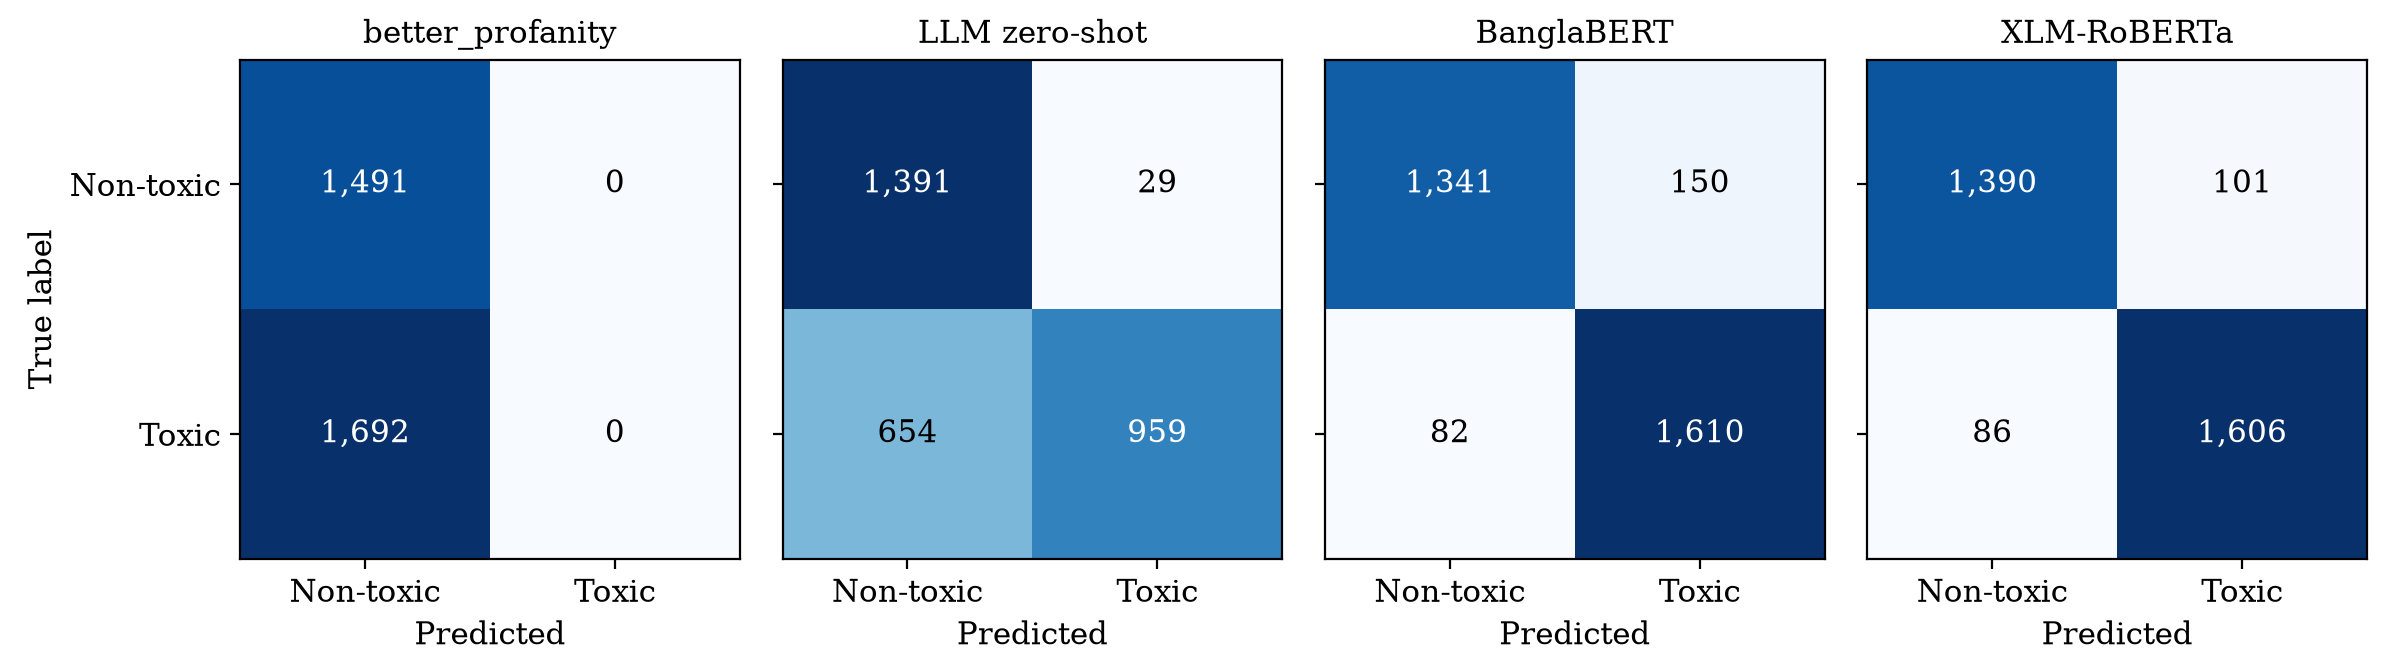
\includegraphics[width=\textwidth]{confusion_matrices.png}
  \caption{Confusion matrices on the test set (first run for the fine-tuned models). Rows are true labels, columns are predictions. The LLM matrix covers the 3,033 comments it classified.}
  \label{fig:cm}
\end{figure}

\begin{table}[H]
  \centering
  \caption{Per-class precision, recall and F1 on the test set, computed from the confusion matrices in Figure~\ref{fig:cm}.}
  \label{tab:perclass}
  \begin{tabular}{llccc}
    \toprule
    \textbf{Model} & \textbf{Class} & \textbf{Precision} & \textbf{Recall} & \textbf{F1} \\
    \midrule
    \multirow{2}{*}{BanglaBERT} & Non-toxic & 0.942 & 0.899 & 0.920 \\
                                & Toxic     & 0.915 & 0.952 & 0.933 \\
    \midrule
    \multirow{2}{*}{XLM-RoBERTa} & Non-toxic & 0.942 & 0.932 & 0.937 \\
                                 & Toxic     & 0.941 & 0.949 & 0.945 \\
    \midrule
    \multirow{2}{*}{LLM zero-shot} & Non-toxic & 0.680 & 0.980 & 0.803 \\
                                   & Toxic     & 0.971 & 0.595 & 0.737 \\
    \bottomrule
  \end{tabular}
\end{table}

The two fine-tuned models make different kinds of errors. BanglaBERT leans towards flagging comments: it misses only 82 of 1,692 toxic comments (4.8\%), but wrongly flags 150 of 1,491 non-toxic ones (10.1\%). XLM-RoBERTa misses a similar number of toxic comments (86, or 5.1\%) while raising a third fewer false alarms (101, or 6.8\%). Its advantage therefore comes mainly from recognising harmless comments more reliably. For a moderation system this matters, because every false alarm means a legitimate comment is hidden or sent for manual review.

\subsection{Training Dynamics}

Figure~\ref{fig:dynamics} shows the training and validation loss and the validation F1-score of a BanglaBERT training run over its five epochs. The training loss falls steadily from 0.26 to 0.03. The validation loss is lowest after the first epoch and then rises to 0.58, while the validation F1-score still improves slightly, from 0.903 to 0.914. The model therefore becomes increasingly over-confident on the examples it gets wrong (overfitting, as measured by the loss), even though the number of correct decisions keeps rising a little. Selecting checkpoints by validation F1 rather than validation loss is therefore appropriate for this task. Fewer epochs, or stronger regularisation, would likely give similar F1-scores at a lower training cost.

\begin{figure}[H]
  \centering
  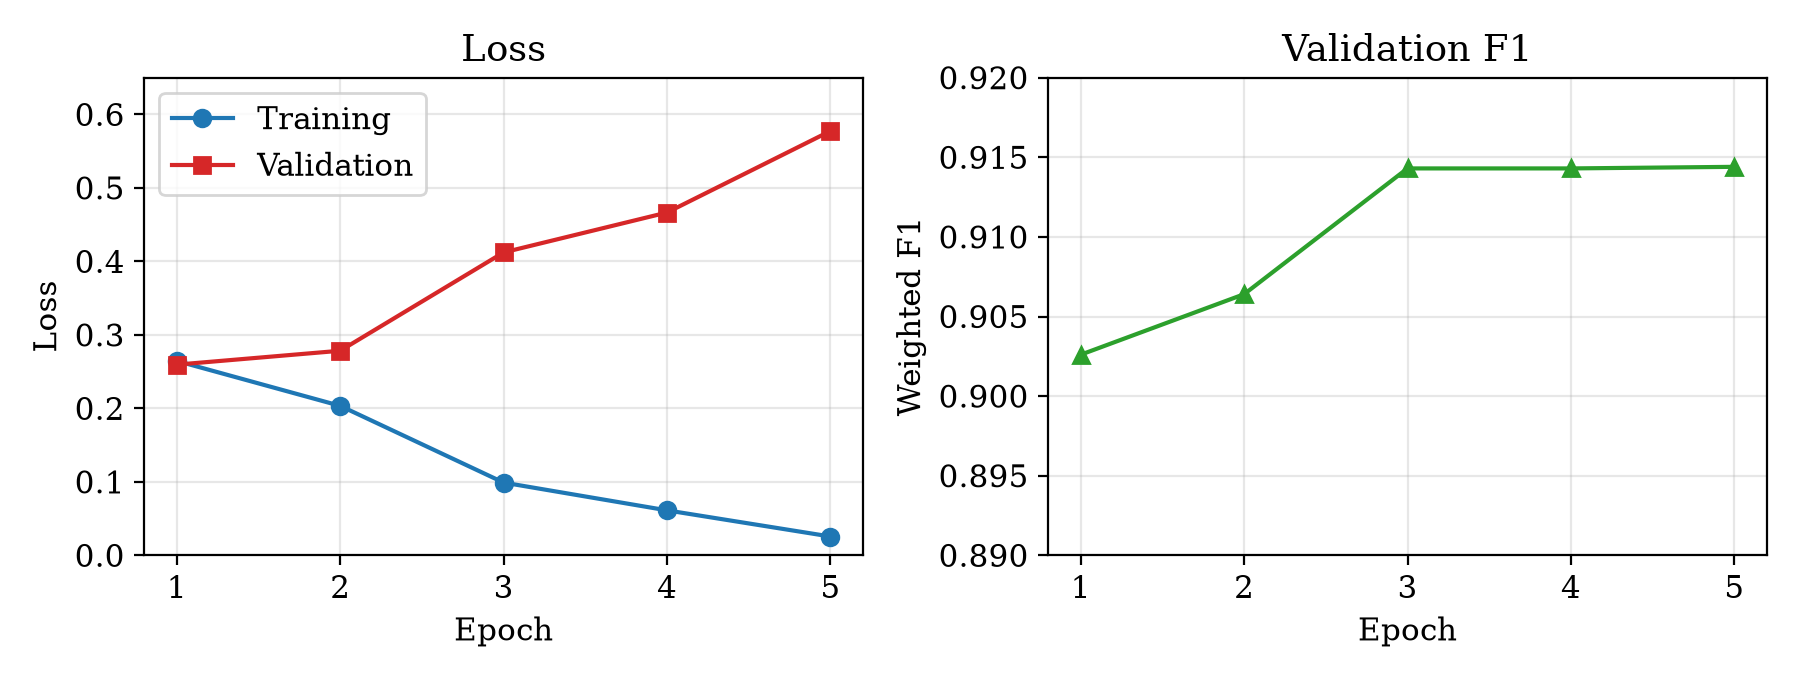
\includegraphics[width=\textwidth]{training_dynamics.png}
  \caption{Training behaviour of BanglaBERT over five epochs (seed 43). The validation loss rises after the first epoch, a sign of overfitting, while the validation F1-score still improves slightly.}
  \label{fig:dynamics}
\end{figure}

\subsection{Effect of Training Data Size}

Figure~\ref{fig:lc} shows the test F1-score when the models are trained on 25\%, 50\% and 100\% of the training data.

\begin{figure}[H]
  \centering
  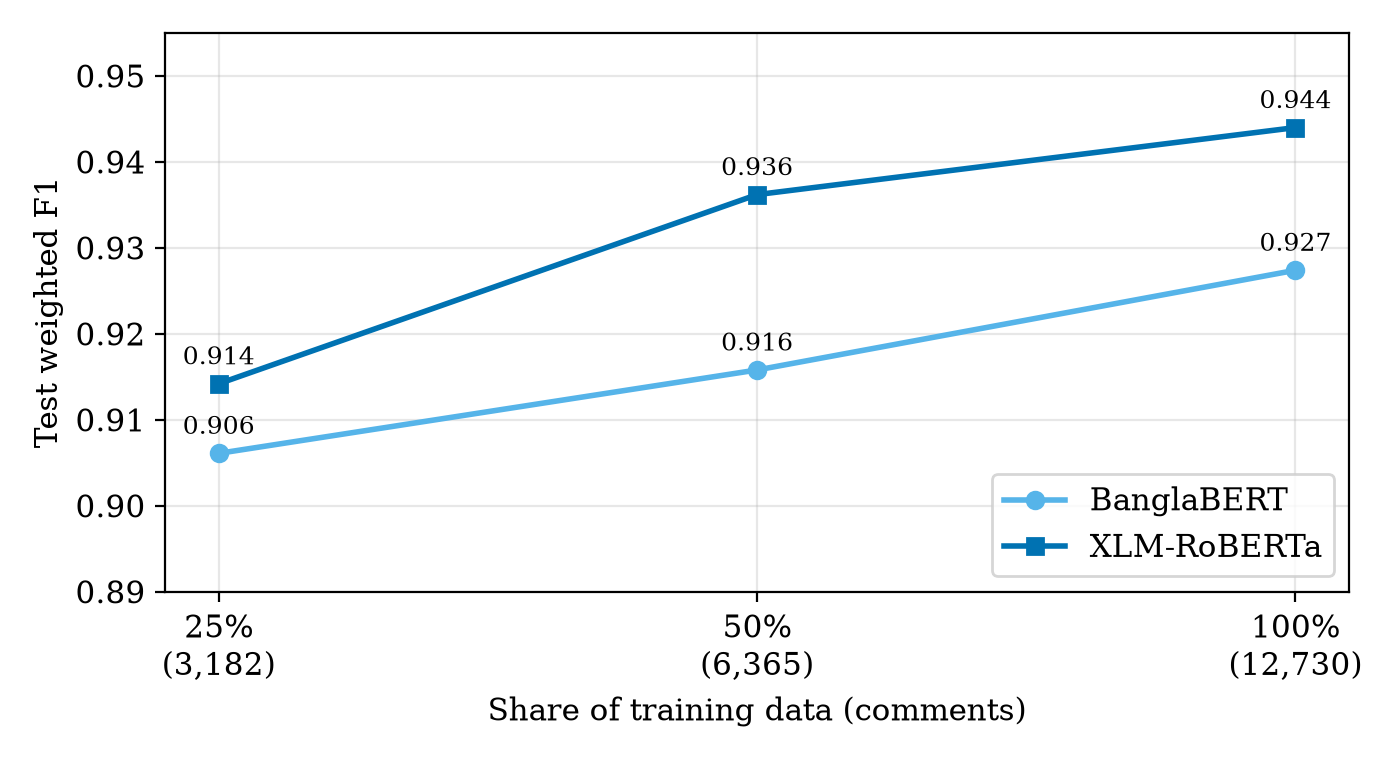
\includegraphics[width=0.85\textwidth]{learning_curves.png}
  \caption{Learning curves: test F1-score of each fine-tuned model against the amount of training data used.}
  \label{fig:lc}
\end{figure}

Three observations stand out. First, both models already perform well with little data: trained on only 3,182 comments (25\%), they reach F1-scores of 0.906 (BanglaBERT) and 0.914 (XLM-RoBERTa), far above the zero-shot LLM. Second, both curves are still rising at 100\%: going from half to all of the data adds 1.2 F1 points for BanglaBERT and 0.8 for XLM-RoBERTa. More labelled data would therefore probably still help, although with diminishing returns. Third, XLM-RoBERTa is ahead at every data size, and XLM-RoBERTa trained on half of the data (0.936) already outperforms BanglaBERT trained on all of it (0.927).

\section{Zero-shot LLM Baseline}
\label{sec:llm}

The LLM classified 3,033 of the 3,183 test comments. The remaining 150 comments (six batches) were not classified because the free tier of the API limits usage to 200,000 tokens per day \cite{groqdocs}. Because the test set is in random order, the missing comments are an essentially random subset, so excluding them should not bias the result noticeably. They are excluded from the LLM's scores rather than counted as errors.

The LLM reaches an F1-score of 0.768. Its behaviour is very different from that of the fine-tuned models (Table~\ref{tab:perclass}). When it labels a comment as toxic, it is almost always right: toxic precision is 0.971, with only 29 false alarms. However, it misses 654 of 1,613 toxic comments, a toxic recall of only 0.595. In other words, the model is very \emph{conservative}: it flags only clearly offensive comments and lets milder insults, trolling and implicit attacks through. Possible explanations include the model's limited exposure to informal Bangla, including slang and spelling variants, differences between the model's notion of toxicity and the dataset's annotation guidelines (which count trolling and mild insults as toxic), and the absence of any examples in the prompt.

The LLM is also slow in this setup: 2.6 comments per second, compared with about 180 for the fine-tuned models. Classifying the full test set took roughly 20 minutes and used almost the entire daily free-tier allowance, and the approach depends on an external service. These factors make zero-shot prompting impractical for large-scale moderation, although it may still be useful as a quick, high-precision first filter where no labelled data is available.

\section{Inference Efficiency}

Figure~\ref{fig:speed} plots accuracy against speed. The fine-tuned models are both the most accurate and the fastest. They classify about 180 comments per second on a single free GPU, roughly 70 times faster than the LLM. Once trained, they also run without any external service or per-request cost. The lexicon filter is relatively slow, at 21 comments per second, probably because it checks every word against its list in pure Python.

\begin{figure}[H]
  \centering
  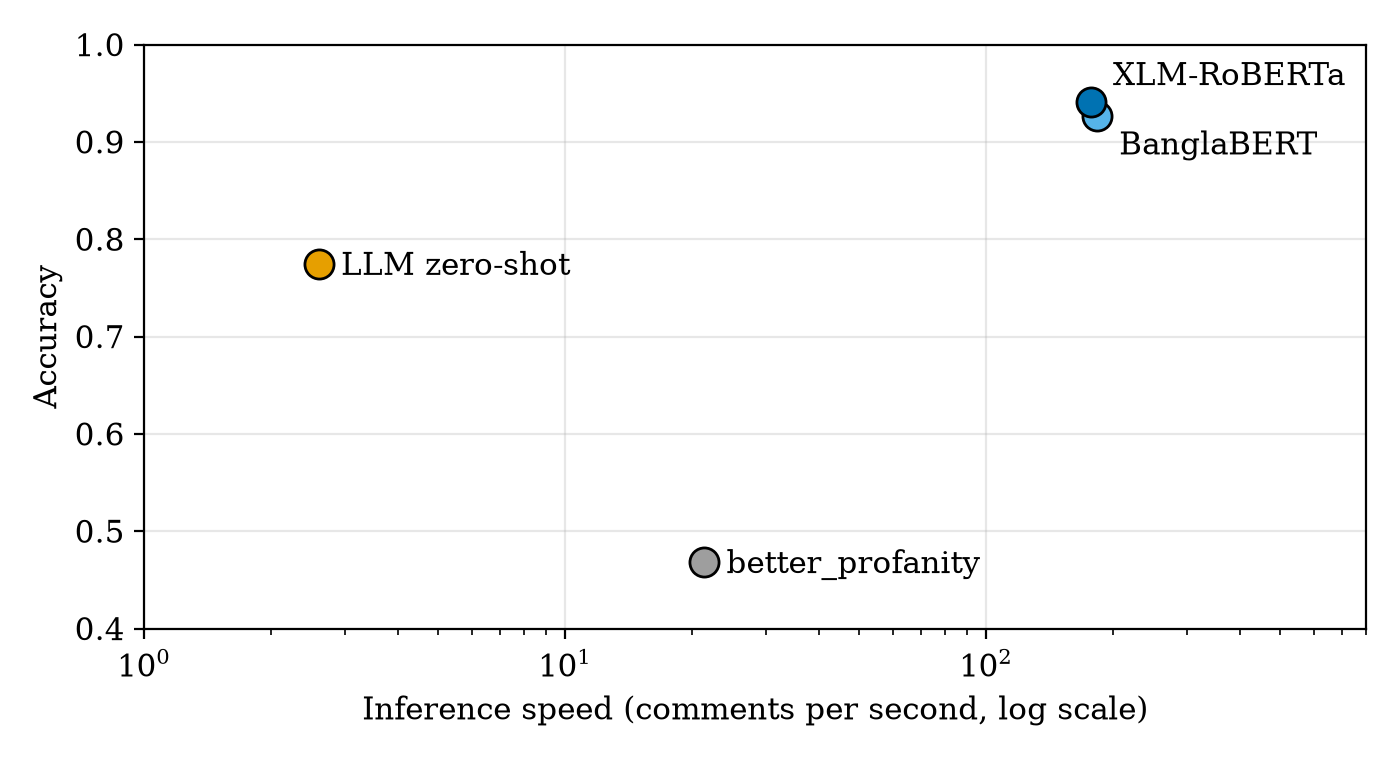
\includegraphics[width=0.85\textwidth]{accuracy_vs_speed.png}
  \caption{Accuracy against inference speed. The fine-tuned models are both the most accurate and the fastest. Fine-tuned model accuracy is from the first run.}
  \label{fig:speed}
\end{figure}

\section{Comparison with Previous Work}

Belal et al. \cite{belal2023toxic} reported a binary toxic-versus-non-toxic accuracy of 89.42\% on the same dataset. The fine-tuned models in this thesis reach a mean accuracy of 92.8\% (BanglaBERT) and 94.3\% (XLM-RoBERTa). The results are not directly comparable, because the train/test splits, preprocessing (this thesis removes duplicate comments) and evaluation details differ. Nevertheless, they indicate that fine-tuning modern pretrained transformers is a strong approach for this dataset.

\section{Answers to the Research Questions}

\textbf{RQ1: How accurately can fine-tuned transformers detect toxic Bangla comments?} Very accurately. Both models exceed an F1-score of 0.92 and miss only about 5\% of toxic comments, and their results vary little between runs.

\textbf{RQ2: Does the Bangla-specific model outperform the multilingual one?} No. XLM-RoBERTa outperforms BanglaBERT by about 1.5 F1 points, consistently across seeds and at every training-data size, mainly by raising fewer false alarms. A likely explanation is that XLM-RoBERTa was pretrained on far more data overall (2.5 TB of filtered web text) and has a larger vocabulary, so it may have seen more of the informal, varied language found in social-media comments. The result shows that being language-specific does not by itself guarantee better performance, although a larger Bangla model such as \texttt{csebuetnlp/banglabert} \cite{bhattacharjee2022banglabert} may close the gap.

\textbf{RQ3: How does a zero-shot LLM compare?} It is clearly worse, with an F1-score of 0.768 against 0.928--0.943. It is very precise but misses about 41\% of toxic comments, and it is about 70 times slower in this setup. Fine-tuning on a few thousand labelled examples remains the better choice when labelled data is available.

\textbf{RQ4: Is a lexicon filter adequate?} No. An off-the-shelf English profanity filter did not flag a single toxic comment in the Bangla test set.

\textbf{RQ5: How does performance depend on training data size?} Performance rises steadily with more data, but even a quarter of the training set (about 3,200 comments) gives F1-scores above 0.90. The curves have not flattened at 12,730 comments, so collecting more labelled data would probably bring further, smaller gains.

\chapter{Conclusion and Future Work}
\justifying

\section{Conclusion}

This thesis compared four approaches to detecting toxic Bangla comments under one controlled protocol: an English lexicon filter, the Bangla-specific BanglaBERT, the multilingual XLM-RoBERTa, and a zero-shot large language model. All were evaluated on the same 3,183 held-out comments from the Multi-labeled Bengali Toxic Comments dataset. Model selection used a separate validation split, and the fine-tuned models were each trained three times.

Fine-tuned transformers are by far the most effective approach. XLM-RoBERTa achieves the best weighted F1-score, 0.943, and BanglaBERT reaches 0.928. Both miss only about 5\% of toxic comments, XLM-RoBERTa raises a third fewer false alarms, and both classify around 180 comments per second on a free GPU. Even with a quarter of the training data, both models exceed an F1-score of 0.90. The zero-shot LLM reaches an F1-score of 0.768. It rarely raises false alarms, but it misses many toxic comments and is much slower and dependent on an external service. The English lexicon filter is ineffective for Bangla. These results suggest that, for Bangla content moderation, collecting a moderate amount of labelled data and fine-tuning a pretrained multilingual transformer is currently the most accurate and cost-effective strategy.

\section{Limitations}

\begin{itemize}
  \item \textbf{Single dataset.} All experiments use one dataset from one collection effort, so the models may not generalise equally well to other platforms, topics or time periods.
  \item \textbf{Binary labels.} The six toxicity types were merged into one label. The thesis does not evaluate how well each type (for example threats or religious hate) is detected.
  \item \textbf{Bangla script only.} The dataset contains comments in Bangla script. Romanised Bangla (``Banglish'') and code-mixed Bangla--English, which are common on social media, were not studied.
  \item \textbf{Incomplete LLM coverage.} Because of free-tier API limits, the LLM was scored on 3,033 of 3,183 test comments, and only one LLM and one prompt were tested.
  \item \textbf{No hyperparameter search.} Standard fine-tuning settings were used for both models. Tuning them could change the margins between the models.
  \item \textbf{Few runs.} Three runs per model give an estimate of variability but are too few for formal significance testing.
\end{itemize}

\section{Future Work}

\begin{itemize}
  \item \textbf{Stronger Bangla models.} Evaluate \texttt{csebuetnlp/banglabert} \cite{bhattacharjee2022banglabert} and larger multilingual models such as XLM-RoBERTa-large.
  \item \textbf{Multi-label classification.} Predict the six toxicity types directly, which supports more nuanced moderation policies.
  \item \textbf{More datasets.} Evaluate across datasets, for example by training on this dataset and testing on BD-SHS \cite{romim2022bdshs}, to measure generalisation.
  \item \textbf{Romanised and code-mixed text.} Collect or adapt data in Banglish and mixed Bangla--English.
  \item \textbf{Better LLM use.} Test few-shot prompting with labelled examples, prompts that include the annotation guidelines, and other LLMs, and use LLMs to generate additional training data.
  \item \textbf{Explainability.} Highlight the words that drive each prediction, to help moderators understand and trust the system.
\end{itemize}


% ===========================================================================
% References (BibTeX)
% ===========================================================================
\clearpage
\phantomsection
\addcontentsline{toc}{chapter}{References}
\bibliographystyle{unsrtnat}
\bibliography{ref}

\end{document}
